\documentclass[11pt,a4paper,notitlepage]{article}

\usepackage{styles/reportstyle}

\graphicspath{{images/}}

%\syntaxonly

\title{
    
\includegraphics[scale=0.15]{feuplogo.jpg}\\
    \vspace{0.5\baselineskip}
    \huge Simulação de um sistema de reserva de lugares\\
    \large Implementação de uma arquitetura cliente/servidor baseada em FIFOs\\
}

\author{
    Bruno Carvalho    \\\text{up201606517@fe.up.pt}
    \and
    João Alves        \\\text{up201605236@fe.up.pt}
    \and
    João Agulha       \\\text{up201607930@fe.up.pt}
}

\begin{document}
\maketitle
\tableofcontents
\pagebreak

\section{Estrutura das Mensagens}
\label{sec:structure}

Como não foi especificado o formato das mensagens a partilhar
na \emph{fifo ansXXXXX}, decidimos usar dois formatos, um para
reservas bem sucedidas e outro para reservas mal sucedidas.

Se o \emph{client} for compilado em modo \textit{debug} (ver
\emph{debug.h}) então as mensagens recebidas no \emph{fifo ansXXXXX}
são escritas em \emph{stdout}.\\

\begin{enumerate}
\item Para reservas de $N$ lugares bem sucedidas:\\
\msg{SUCCESS \textit{seat1} \textit{seat2} ... \textit{seatN}}
\item Para reservas mal sucedidas:\\
\msg{ERROR \textit{code}}\\
\end{enumerate}

% Meter imagens aqui ...
\begin{figure}[htbp]
\centering
\label{fig:ans}
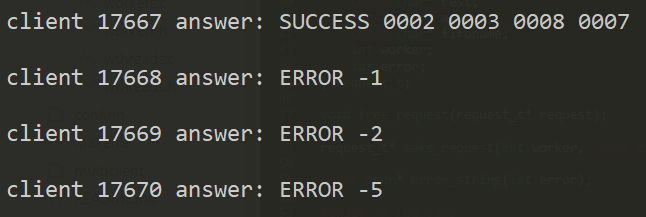
\includegraphics[height=8em]{ans.png}
\caption{Mensagens exemplo, ecoadas pelo \emph{client} no terminal}
\end{figure}

\section{Mecanismos de Sincronização}
\label{sec:sync}

Usamos mecanismos de sincronização no acesso aos \emph{seats}
pelas bilheteiras e no acesso à \emph{queue} de mensagens entre
o \emph{thread} principal e as bilheteiras.

Para salvaguardar do acesso simultâneo aos \emph{seats},
cada \emph{seat} tem um \emph{mutex} associado. O \emph{mutex} $i$
do \emph{seat} $i$ serve de fila de acesso unitário a todas
as bilheteiras a tentar aceder a esse mesmo \emph{seat}.
Como são usados \emph{mutex} POSIX, não há garantia de espera
limitada.

Para gerir a \emph{queue} de mensagens, é usado um esquema
à semelhança do \textit{Reader-Writer} estudado nas aulas.
São usados dois \emph{mutexes} para gerir a permissão de
escrita e de leitura, cada um com o seu semáforo auxiliar:
o primeiro -- \emph{not\_full\_sem} -- que conta o número de
espaços disponíveis para escrita, e outro -- \emph{not\_empty\_sem}
-- que conta o número de mensagens por ler. Um escritor
(o \emph{thread} principal) que queira escrever tem de tomar
posse do \emph{mutex} de escrita e, se necessário, esperar
no primeiro semáforo por um espaço livre; já um leitor (uma bilheteira)
tem de tomar posse do \emph{mutex} de leitura e, se necessário,
esperar no segundo semáforo por uma mensagem nova.

A especificação requer que a \emph{queue} de mensagens
tenha tamanho unitário, mas a implementação
suporta um \emph{queue} de qualquer tamanho,
vários leitores e escritores.\\

% Meter 2 imagens aqui...
\begin{figure}[htbp]
\centering
\begin{minipage}{.5\textwidth}
\centering
\label{fig:ans}
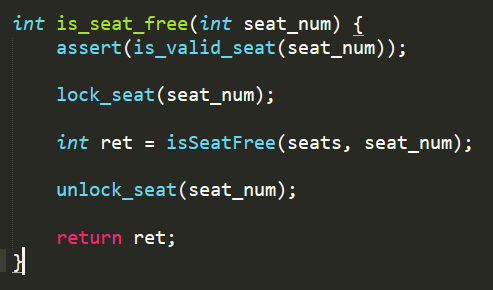
\includegraphics[height=9em]{is_seat_free.png}
\captionof{figure}{Acesso aos \emph{seats}}
\end{minipage}%
\begin{minipage}{.5\textwidth}
\centering
\label{fig:ans}
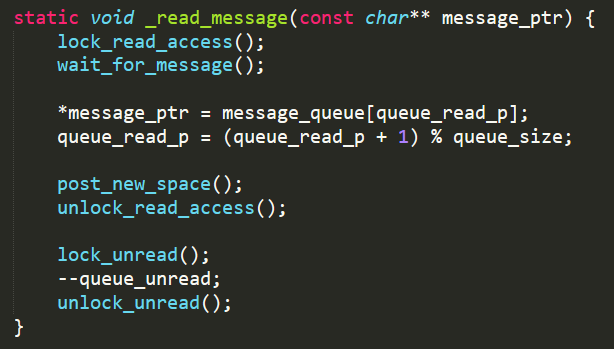
\includegraphics[height=11em]{read_message.png}
\captionof{figure}{Acesso à \emph{queue}}
\end{minipage}
\end{figure}

\section{Encerramento das Bilheteiras}
\label{sec:workers}

O único escritor do \emph{queue} é o \emph{thread} principal,
e este escreve as mensagens lidas do \emph{fifo requests} diretamente
para esse \emph{queue} sem qualquer processamento prévio.
Para terminar as bilheteiras, o \emph{thread} principal escreve
no \emph{queue} uma mensagem específica definida pela implementação,
de momento \textup{WORKER\_EXIT}, por cada bilheteira.

Por sua vez, as bilheteiras que lêem esta mensagem identificam-na
e terminam a sua execução de forma natural.

A terminação natural do servidor por \emph{timeout} ou por cancelamento
no terminal (\textup{\mbox{Ctrl-C}}, ...) são equivalentes,
e chamam \textbf{exit}
diretamente. Existem vários \textbf{atexit handlers} instalados,
o primeiro a ser executado fecha e destrói imediatamente o
\emph{fifo requests}, o segundo envia as mensagens de terminação às
bilheteiras e espera que elas terminem a execução normalmente (o que
pode demorar tendo em consideração \textit{DELAY()}). Os restantes
libertam toda a memória reservada para as estruturas de dados usadas,
\emph{strings} guardadas, \emph{mutexes}, etc.\\

% Meter 2 imagens aqui...
\begin{figure}[htbp]
\centering
\begin{minipage}{.5\textwidth}
\centering
\label{fig:ans}
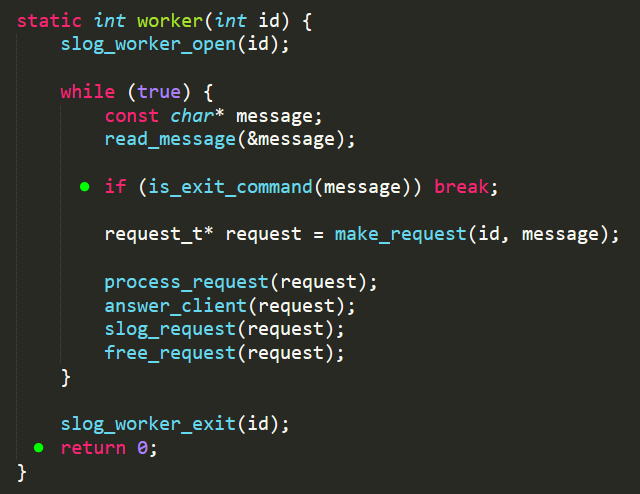
\includegraphics[height=14em]{worker.png}
\captionof{figure}{Bilheteiras identificam mensagens}
\end{minipage}%
\begin{minipage}{.5\textwidth}
\centering
\label{fig:ans}
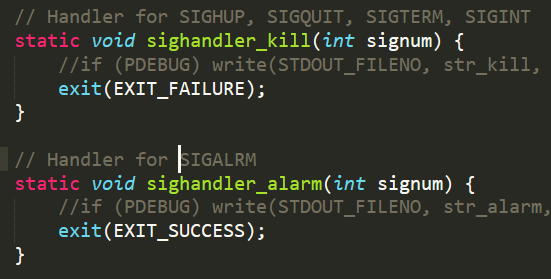
\includegraphics[height=9em]{sighandlers.png}
\captionof{figure}{Signal Handlers}
\end{minipage}
\end{figure}

\end{document}